\documentclass{beamer}
\usetheme[height=7mm]{Rochester}
\usepackage{listings}

%\usefonttheme{serif}

\usepackage[T1]{fontenc}
\usepackage{inconsolata}

\usepackage[absolute,overlay]{textpos} 
\newenvironment{reference}[2]{% 
  \begin{textblock*}{\textwidth}(#1,#2) 
      \tiny\bgroup\color{red!50!black}}{\egroup\end{textblock*}} 


\begin{document}

%%%%%%%%%%%%%%%%%%%%%%%%%%%%%%%%%%%%%%%%%%%%%%%%%%%%%%%%%%%%%%%%%%%%%%%%%%%%%%%%
\title{Profile and reorder code execution in Geant4 to increase performance}
\subtitle{A Google Summer of Code Project}
\author{Stathis Kamperis}
\institute{
  Department of Physics\\
  Aristotle University of Thessaloniki\\
  Greece\\[1ex]
  \texttt{ekamperi@gmail.com}
}
\date{July, 2012}

\begin{frame}[plain]
  \titlepage
\end{frame}


%%%%%%%%%%%%%%%%%%%%%%%%%%%%%%%%%%%%%%%%%%%%%%%%%%%%%%%%%%%%%%%%%%%%%%%%%%%%%%%%
\begin{frame}{Overview}

Geant4
\begin{itemize}
  \item Large source code base
  \item Lots of classes
  \item Highly conditionalized code
  \item Complex numerical calculations
\end{itemize}

Full CMS
\begin{itemize}
\item Complex geometry and physics
\end{itemize}

\begin{center}
\fcolorbox{red}{white}{Very low visibility to the runtime aspects of the simulations}
\end{center}
\end{frame}

%%%%%%%%%%%%%%%%%%%%%%%%%%%%%%%%%%%%%%%%%%%%%%%%%%%%%%%%%%%%%%%%%%%%%%%%%%%%%%%%
\begin{frame}{Profiling targets}
\begin{itemize}
\item Full CMS experiment
\item Simplified Calorimeter
\begin{itemize}
\item Faster initialization, faster profiling cycles
\item Simpler Geometry
\begin{itemize}
\item Useful for examining how (lack of complex) geometry affects performance
\end{itemize}
\end{itemize}
\item Examples bundled with Geant4
\end{itemize}
\end{frame}

%%%%%%%%%%%%%%%%%%%%%%%%%%%%%%%%%%%%%%%%%%%%%%%%%%%%%%%%%%%%%%%%%%%%%%%%%%%%%%%%
\begin{frame}{Profiling tools}

\textcolor{blue}{Ported Geant4 to Solaris 11/x64}

\begin{itemize}
\item DTrace
\begin{itemize}
\item A dynamic tracing framework
\item Available also in Mac OSX (an officially supported platform by Geant4)
\item Fine-grained profiling
\end{itemize}
\item mdb (Modular debugger)
\item cputrack
\begin{itemize}
\item Access CPU performance counters
\item data cache misses, instruction cache misses, branch mispredictions, ...
\end{itemize}
\item libumem
\begin{itemize}
\item Useful for debugging memory problems (leaks, corruptions, etc)
\item As simple as running: LD\_PRELOAD=libumem.so.1 ./a.out
\item Can be used in conjuction with mdb \(::findleaks, ::umem\_verify, ...\)
\end{itemize}
\end{itemize}
\end{frame}

%%%%%%%%%%%%%%%%%%%%%%%%%%%%%%%%%%%%%%%%%%%%%%%%%%%%%%%%%%%%%%%%%%%%%%%%%%%%%%%%
\begin{frame}{Profiling tools - cont.}
\begin{itemize}
\item pbind (to bind profiled process to a specific CPU)
\item A pseudo device driver to invalidate CPU caches on demand
\item Visualisation tools and Statistics
\begin{itemize}
\item gnuplot, ggplot2, R
\end{itemize}
\end{itemize}
\end{frame}

%%%%%%%%%%%%%%%%%%%%%%%%%%%%%%%%%%%%%%%%%%%%%%%%%%%%%%%%%%%%%%%%%%%%%%%%%%%%%%%%
\begin{frame}{Profiling tools - Alternatives}

\textcolor{blue}{Not propagandizing in favor of Solaris}

\vspace{5mm}

Alternatives for Linux users:

\begin{itemize}
\item DTrace $\rightarrow$ SystemTap
\item mdb $\rightarrow$ gdb
\item cputrack $\rightarrow$ perf, cachegrind
\item libumem $\rightarrow$ valgrind
\item pbind $\rightarrow$ taskset
\end{itemize}

The rest are common for both platforms (visualisation and statistics)

\end{frame}

%%%%%%%%%%%%%%%%%%%%%%%%%%%%%%%%%%%%%%%%%%%%%%%%%%%%%%%%%%%%%%%%%%%%%%%%%%%%%%%%
\begin{frame}{DTrace}

\begin{itemize}
\item pid provider
\item Flamegraphs
\item USDT (user-level statically defined tracing)
\item Speculative tracing
\item All of the above combined
\end{itemize}
\end{frame}

%%%%%%%%%%%%%%%%%%%%%%%%%%%%%%%%%%%%%%%%%%%%%%%%%%%%%%%%%%%%%%%%%%%%%%%%%%%%%%%%
\begin{frame}{DTrace - pid provider}

\textcolor{blue}{Definition} pid provider allows for tracing of the entry and
return of any function in a user process

\vspace{5mm}

The pid provider has no probe effect when probes are not enabled.
\end{frame}

%%%%%%%%%%%%%%%%%%%%%%%%%%%%%%%%%%%%%%%%%%%%%%%%%%%%%%%%%%%%%%%%%%%%%%%%%%%%%%%%

\begin{frame}[fragile]{DTrace - pid provider 1}
\textcolor{blue}{How many times does the {\tt G4Allocator} grow in size during 100 simulated events ?}

\lstset{frame=single, columns=flexible}
\lstset{basicstyle=\tiny\ttfamily}
\begin{lstlisting}
# dtrace -n '
pid$target::*G4AllocatorPool*Grow*:entry
{
    @ = count();
}' -c '/home/stathis/geant4.9.5.p01/bin/full_cms ./bench1_100.g4'

             5921
\end{lstlisting}

\textcolor{blue}{How much time do the above resizes consume ?}

\lstset{frame=single, columns=flexible}
\lstset{basicstyle=\tiny\ttfamily}
\begin{lstlisting}
dtrace -n '
pid$target::*G4AllocatorPool*Grow*:entry
{
    self->ts = vtimestamp;
}

pid$target::*G4AllocatorPool*Grow*:return
/self->ts/
{
    @ = sum((vtimestamp - self->ts)/1000);
    self->ts = 0;
}' -c '/home/stathis/geant4.9.5.p01/bin/full_cms ./bench1_100.g4'
             4859  # ~5 msec
\end{lstlisting}
\end{frame}

%%%%%%%%%%%%%%%%%%%%%%%%%%%%%%%%%%%%%%%%%%%%%%%%%%%%%%%%%%%%%%%%%%%%%%%%%%%%%%%%
\begin{frame}[fragile]{DTrace - pid provider 2}
\textcolor{blue}{How do we skip the initialization part of Geant4/Full CMS ?}
\begin{itemize}
\item Use a predicate that checks whether we are inside the DoEventLoop()
\end{itemize}

\lstset{frame=single, columns=flexible}
\lstset{basicstyle=\tiny\ttfamily}
\begin{lstlisting}
dtrace -n '
BEGIN
{
    tracing = 0;
}

pid$target::*DoEventLoop*:entry  { tracing = 1; }
pid$target::*DoEventLoop*:return { exit(0);     }

someprobe
/tracing != 0/
{
    ...
}
' -c '/home/stathis/geant4.9.5.p01/bin/full_cms ./bench_100.g4'
\end{lstlisting}

\end{frame}

%%%%%%%%%%%%%%%%%%%%%%%%%%%%%%%%%%%%%%%%%%%%%%%%%%%%%%%%%%%%%%%%%%%%%%%%%%%%%%%%
\begin{frame}{USDT (user-level statically defined tracing)}
\textcolor{blue}{Allows to place custom probe points in application code}
\begin{itemize}
\item Available both in development and production builds
\begin{itemize}
\item No need to recompile with a debug flag set
\end{itemize}
\item DTrace dynamically activates the probes when asked
\begin{itemize}
\item By dynamically modifying the instructions of the profiled app
\end{itemize}
\item Negligible overhead when not in use (a few NOPs)
\item Take advantage of DTrace rich reporting capabilities (aggregations)
\end{itemize}
\end{frame}

%%%%%%%%%%%%%%%%%%%%%%%%%%%%%%%%%%%%%%%%%%%%%%%%%%%%%%%%%%%%%%%%%%%%%%%%%%%%%%%%
\begin{frame}{USDT (user-level statically defined tracing)}
\begin{itemize}
\item \textcolor{blue}{simple\_provider.d}: defines the provider probes and argument-
linked into the module binary at link time
\item \textcolor{blue}{simple\_provider.h}: defines the structure passed from Geant4
to DTrace at run time
\item \textcolor{blue}{G4SmartTrackStack.cc}: uses hooks at the end of each push pop operation
to fire the corresponding DTrace probes
\end{itemize}
\end{frame}

%%%%%%%%%%%%%%%%%%%%%%%%%%%%%%%%%%%%%%%%%%%%%%%%%%%%%%%%%%%%%%%%%%%%%%%%%%%%%%%%
\begin{frame}[fragile]{USDT - Example 1}
\lstset{basicstyle=\tiny\ttfamily}

\textcolor{blue}{Objective} Everytime we \textit{push} a track to the track manager or we \textit{pop} one from it,
dump the sizes of all stacks.

\lstset{frame=single, columns=flexible}
\begin{lstlisting}
# dtrace -qn '
simple$target:::
{
    printf("%s track=%d size=%d\n", probefunc, arg0, arg1);
}'
-c '/home/stathis/geant4.9.5.p01/bin/mainStatAccepTest ./exercise.g4' | c++filt -np
...
G4SmartTrackStack::PushToStack track=0 size=1
G4SmartTrackStack::PopFromStack track=0 size=0
G4SmartTrackStack::PushToStack track=2 size=1
G4SmartTrackStack::PushToStack track=2 size=2
G4SmartTrackStack::PushToStack track=2 size=3
G4SmartTrackStack::PushToStack track=0 size=1
...
G4SmartTrackStack::PopFromStack track=2 size=446
G4SmartTrackStack::PopFromStack track=2 size=445
G4SmartTrackStack::PopFromStack track=2 size=444
G4SmartTrackStack::PopFromStack track=2 size=443
\end{lstlisting}
\end{frame}

%%%%%%%%%%%%%%%%%%%%%%%%%%%%%%%%%%%%%%%%%%%%%%%%%%%%%%%%%%%%%%%%%%%%%%%%%%%%%%%%
\begin{frame}[fragile]{USDT - Example 2}
\lstset{basicstyle=\tiny\ttfamily}

\textcolor{blue}{Objective} Print the distribution of stack sizes for unclassified particles
(primaries + any particle not beloning to the set ${n^0, e^-,\gamma, e^+}$

\lstset{frame=single, columns=flexible}
\begin{lstlisting}
# dtrace -qn '
simple$target:::
/arg0==1/
{
    @["distribution of 1st stack's size"] = quantize(arg1);
}' -c '/home/stathis/geant4.9.5.p01/bin/mainStatAccepTest ./exercise.g4'
^C
  distribution of 1st stack's size
           value  ------------- Distribution ------------- count
              -1 |                                         0
               0 |                                         111
               1 |                                         308
               2 |@                                        963
               4 |@                                        2241
               8 |@@                                       3193
              16 |@@@                                      4452
              32 |@@@@@                                    7700
              64 |@@@@@@@@@@                               15574
             128 |@@@@@@@@@@@@@@@                          23497
             256 |@@@                                      4459
             512 |                                         0
\end{lstlisting}
\end{frame}

%%%%%%%%%%%%%%%%%%%%%%%%%%%%%%%%%%%%%%%%%%%%%%%%%%%%%%%%%%%%%%%%%%%%%%%%%%%%%%%%
\begin{frame}{USDT - Example 3}

\textcolor{blue}{Objective} Visualize the size of stacks and the total energy of their particles

\vspace{1mm}

The following graph is from a simulation of 2 events in Full CMS:

\begin{center}
  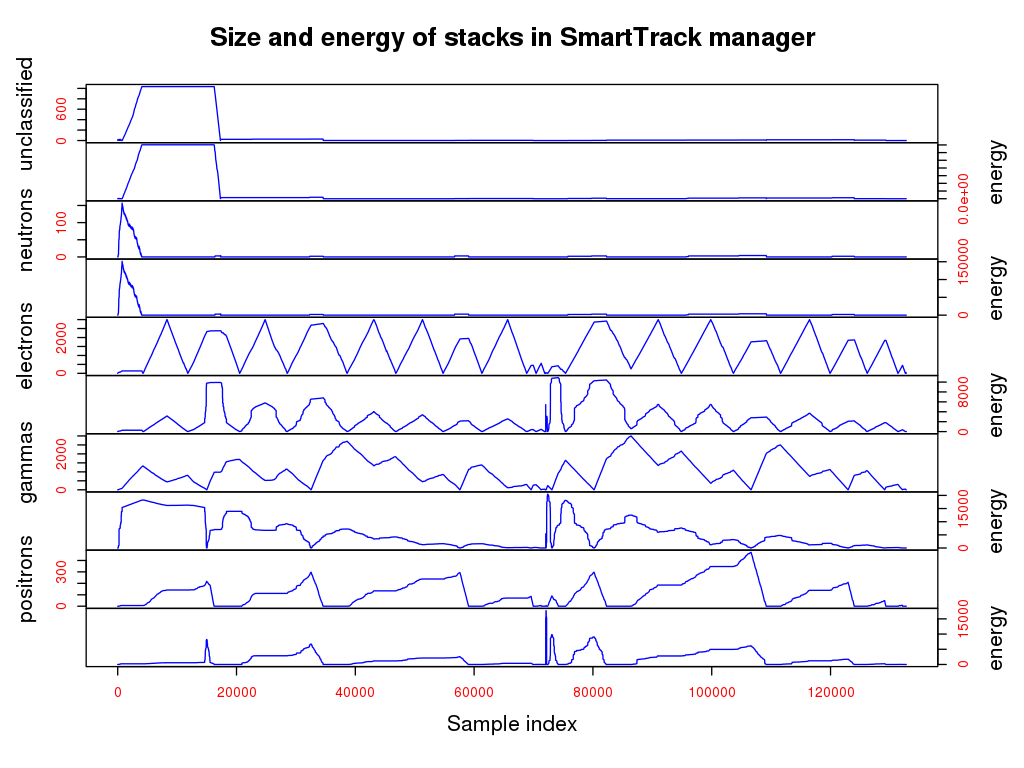
\includegraphics[width=0.8\textwidth]{smarttracksize-ts-2evts-energy.png}
\end{center}
\end{frame}

%%%%%%%%%%%%%%%%%%%%%%%%%%%%%%%%%%%%%%%%%%%%%%%%%%%%%%%%%%%%%%%%%%%%%%%%%%%%%%%%
\begin{frame}{Speculative tracing - Introduction}
\begin{reference}{4mm}{85mm}
From DTrace guide
\end{reference} 
\textcolor{blue}{Definition} The ability to tentatively trace data and then later decide whether to commit
the data to a tracing buffer or discard it.
\end{frame}

%%%%%%%%%%%%%%%%%%%%%%%%%%%%%%%%%%%%%%%%%%%%%%%%%%%%%%%%%%%%%%%%%%%%%%%%%%%%%%%%
\begin{frame}{Speculative tracing - A real use case}

\textcolor{blue}{Problem} Some {\tt ProcessOneEvent()} need more than average time to complete

\begin{center}
  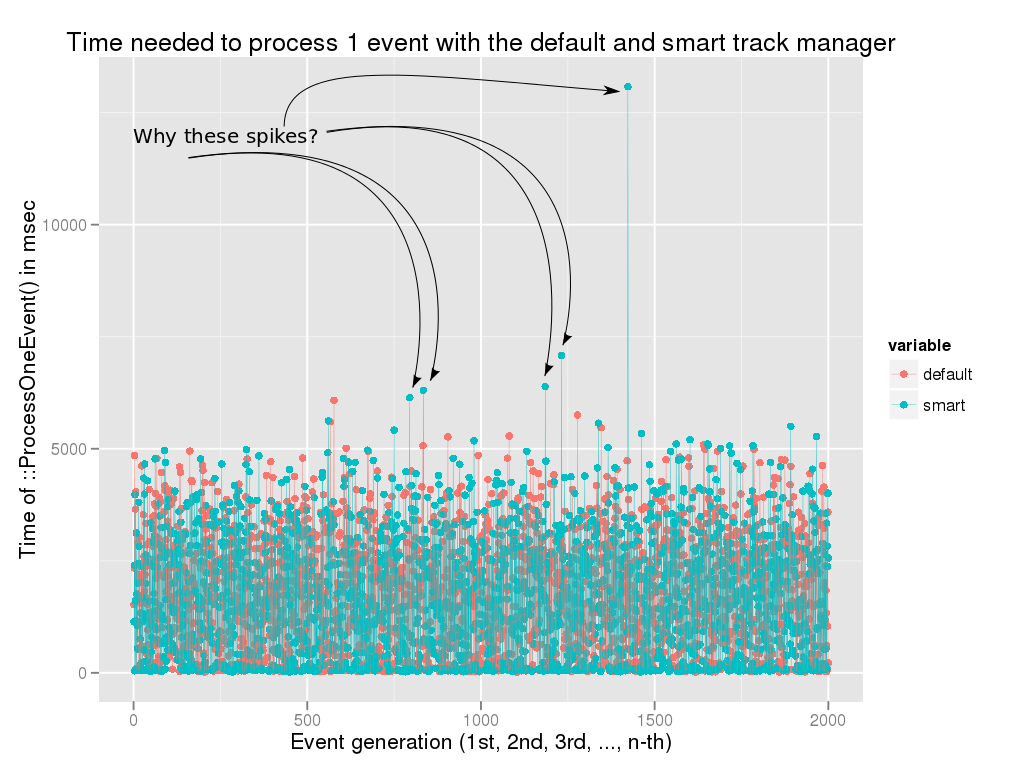
\includegraphics[width=0.8\textwidth]{evts1-arrows.png}
\end{center}
\end{frame}

%%%%%%%%%%%%%%%%%%%%%%%%%%%%%%%%%%%%%%%%%%%%%%%%%%%%%%%%%%%%%%%%%%%%%%%%%%%%%%%%
\begin{frame}{Speculative tracing - A real use case}
\textcolor{blue}{Strategy} We are going to trace all {\tt ProcessOneEvent()} calls, but commit to our tracing
buffer \textit{only} those that behave bad.
\end{frame}

%%%%%%%%%%%%%%%%%%%%%%%%%%%%%%%%%%%%%%%%%%%%%%%%%%%%%%%%%%%%%%%%%%%%%%%%%%%%%%%%
\begin{frame}[fragile]{Speculative tracing - A real use case cont.}
\lstset{basicstyle=\tiny\ttfamily}
\lstset{frame=single, columns=flexible}
\begin{lstlisting}
pid$target::*G4EventManager*ProcessOneEventEP7G4Event:entry
{
    self->pstart = vtimestamp;
    spec = speculation();
}

simple$target:::
/tracing && spec/
{
    speculate(spec);
    printf("%d %d %d %d %d\n", arg0, arg1, arg2, arg3, arg4);
}

pid$target::-:'$retaddr'
/self->pstart/
{
    self->t = (vtimestamp - self->pstart)/1000000;
    self->pstart = 0;
}

pid$target::-:'$retaddr'
/spec && self->t >= 4500/
{
    commit(spec);
    spec = 0;
}

pid$target::-:'$retaddr'
/spec && self->t < 4500/
{
    discard(spec);
    spec = 0;
}
\end{lstlisting}
\end{frame}

%%%%%%%%%%%%%%%%%%%%%%%%%%%%%%%%%%%%%%%%%%%%%%%%%%%%%%%%%%%%%%%%%%%%%%%%%%%%%%%%
\begin{frame}{Flame graphs}
\textcolor{blue}{Definition} Flame graphs are a visualization method for sampled stack traces

\begin{center}
  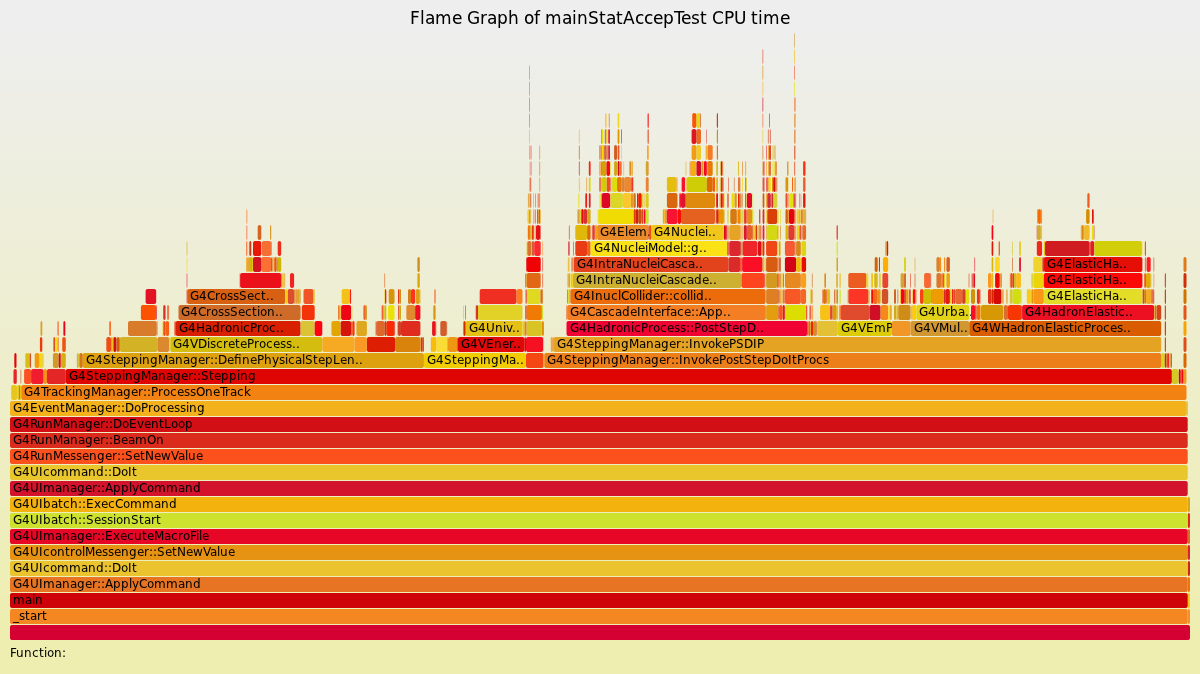
\includegraphics[width=1.0\textwidth]{timeflame.png}
\end{center}
\end{frame}

%%%%%%%%%%%%%%%%%%%%%%%%%%%%%%%%%%%%%%%%%%%%%%%%%%%%%%%%%%%%%%%%%%%%%%%%%%%%%%%%
\begin{frame}{Flame graphs}
\textcolor{blue}{Scope} Anything that can be sampled by DTrace can be visualized as a flame graph
\begin{itemize}
\item Function execution time
\item Data cache misses
\item Instruction cache misses
\item Branch mispredictions
\item Memory allocation sizes
\item ...
\end{itemize}

\begin{reference}{4mm}{85mm}
Developed by Brendan Gregg
\end{reference}
\end{frame}

\begin{frame}{Flame graphs}
\textcolor{blue}{Hints}
\begin{itemize}
\item Identification of hot code-paths
\item The x-axis is the sample population
\item The y-axis is the stack depth
\item The width of a box is proportional to the measured quantity. E.g.,
\begin{itemize}
\item A wide box means that a function either takes a lot of time to complete or
that it is called too often (in either case the probability that its stack trace
is sampled increases)
\end{itemize}
\item The colors are \textit{not} significant (they are picked at random to be "warm")
\end{itemize}
\end{frame}

%%%%%%%%%%%%%%%%%%%%%%%%%%%%%%%%%%%%%%%%%%%%%%%%%%%%%%%%%%%%%%%%%%%%%%%%%%%%%%%%
\begin{frame}{Flame graphs - Validation}
\textcolor{blue}{Problem} How do we know that flame graphs are valid ?

\vspace{5mm}

We picked a function that caused only few cache misses, and made it on purpose
\textit{invalidate all the cpu caches}.

\vspace{5mm}

We then \textit{regenerated} the flame graph and the function's box in the was
\textit{vastly increased}.
\end{frame}

%%%%%%%%%%%%%%%%%%%%%%%%%%%%%%%%%%%%%%%%%%%%%%%%%%%%%%%%%%%%%%%%%%%%%%%%%%%%%%%%
\begin{frame}{Flame graphs - Deltas}

\textcolor{blue}{Definition} A "delta" is a new graph derived
by the subtraction of two flame graphs
\begin{itemize}
\item Examine how a property's value increases or decreases between two versions
of the same application. E.g.,
\begin{itemize}
\item Which functions became faster and which ones slower
\item Which functions cause more instruction cache misses and which ones less
\item ...
\end{itemize}
\item A delta graph consists of two graphs, the flame graph and the cold graph
\end{itemize}

\end{frame}

\begin{frame}{Flame graphs - Deltas - Cold graph}
Example of a cold graph

\begin{center}
  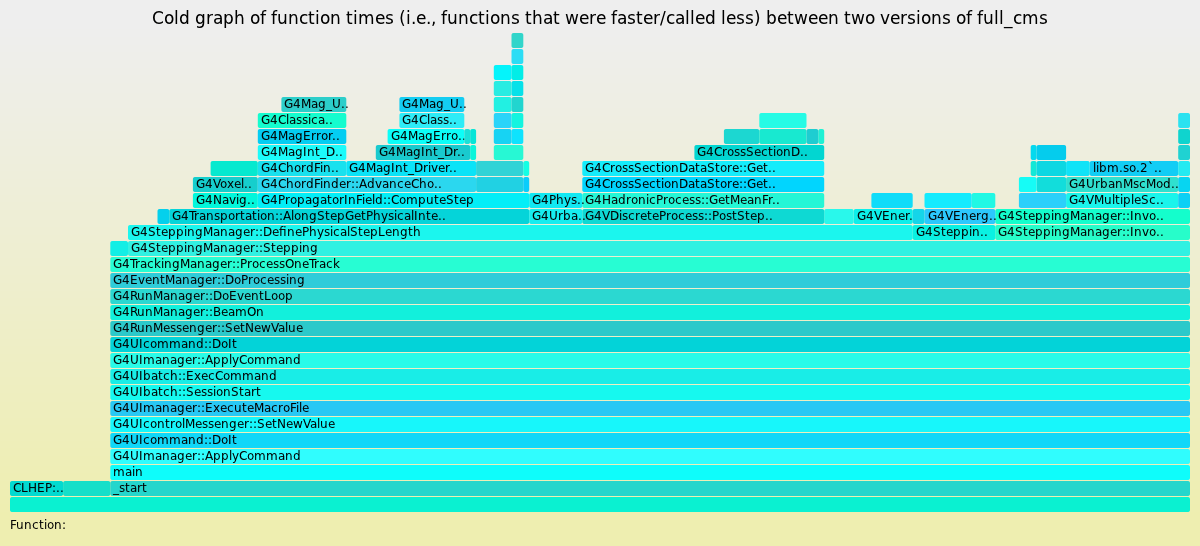
\includegraphics[width=1.0\textwidth]{dec.png}
\end{center}
\end{frame}

%%%%%%%%%%%%%%%%%%%%%%%%%%%%%%%%%%%%%%%%%%%%%%%%%%%%%%%%%%%%%%%%%%%%%%%%%%%%%%%%
\begin{frame}{Particle "bunching"}
\textcolor{blue}{Definition}
Process \textit{same} particle types before switching to another particle type. E.g.,

\begin{equation*}
e^-, e^-, \ldots, e^-, \gamma, \gamma, \ldots, \gamma, \ldots
\end{equation*}

\textcolor{blue}{Why} Better \textit{cache utilisation}

\vspace{5 mm}

Number of stacks we are using: 5

\begin{enumerate}
\item Primary particles + everything not belonging to:
\item Neutrons
\item Electrons
\item Gammas
\item Positrons
\end{enumerate}
\end{frame}

%%%%%%%%%%%%%%%%%%%%%%%%%%%%%%%%%%%%%%%%%%%%%%%%%%%%%%%%%%%%%%%%%%%%%%%%%%%%%%%%
\begin{frame}{Particle "bunching" - Problems}

\textcolor{blue}{Problems}
\begin{itemize}
\item Stacks can grow very large
\begin{itemize}
\item e.g., when processing electrons, the gamma stack explodes, and vice versa
\end{itemize}
\item So we have to restrict them, which leads to another problem
\begin{itemize}
\item What is the optimal size for each one?
\item How much aggressively should we process a track, once it reached its upper limit ?
\end{itemize}
\end{itemize}
\end{frame}

%%%%%%%%%%%%%%%%%%%%%%%%%%%%%%%%%%%%%%%%%%%%%%%%%%%%%%%%%%%%%%%%%%%%%%%%%%%%%%%%
\begin{frame}{Particle "bunching" - Problems cont.}
If we allow \textit{too large} sizes
\begin{itemize}
\item we diverge a lot in terms of geometry (it hurts)
\end{itemize}
If we allow \textit{too small} sizes
\begin{itemize}
\item we switch too often between stacks, and we thrash (it hurts)
\end{itemize}
\end{frame}

%%%%%%%%%%%%%%%%%%%%%%%%%%%%%%%%%%%%%%%%%%%%%%%%%%%%%%%%%%%%%%%%%%%%%%%%%%%%%%%%
\begin{frame}{The end}
\vspace*{\fill}
\begin{center}
Thank you. Questions?
\end{center}
\vspace*{\fill}
\end{frame}

\end{document}
